\section{Empirical Results on Basis Pursuit Denoising \label{appendix:bp}}

We used the implementation of LASSO regression available in sklearn \cite{pedregosa_scikit-learn_2011} to infer sparse subsets of $\{ 1, \dots, 2^{16}\}$ from superposition codes by minimizing the objective
$$
	\quad \frac 1 {2d} \lVert x - F \hat y \rVert_2^2 + 10^{-5} \lVert \hat y \rVert_1
$$
with respect to $\hat y.$ In compressive sensing, this is known as basis pursuit denoising (BPDN). Results are graphed in \Cref{fig:bp}. Compared to the performance of matching pursuit shown in \Cref{fig:mp}, we find that BPDN can recover a subset from even fewer dimensions; around $0.8$ bits per dimension are enough.

\begin{figure}
	\begin{center}
		\centerline{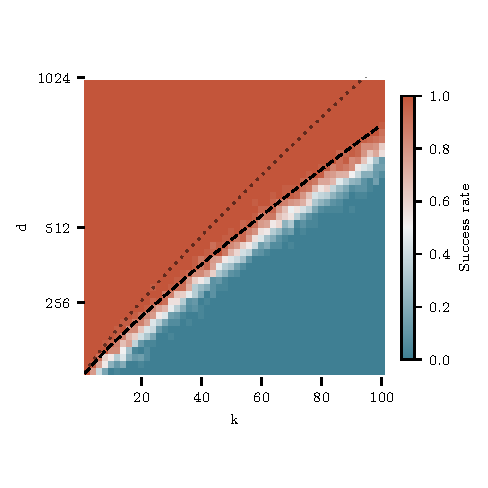
\includegraphics[width=200pt]{figures/bp_decode_new}}
		\caption{Empirical performance of basis pursuit decoding for $N = 2^{16}.$ The bold line shows the relation $d = k \log_2(e N/k),$ and the dotted line shows $d = 0.8 k \log_2(e N/k).$}
		\label{fig:bp}
	\end{center}
\end{figure}
